% Set the author and title of the compiled pdf
\hypersetup{
	pdftitle = {\Title},
	pdfauthor = {\Author}
}

\section{Introduction}

Performance is always an attribute in high demand in computer systems. Even
though processors have become so much more powerful over the last half century,
there's still loads of stuff that we cannot do with current technology, such as
synthesising HD video in realtime, or computing realistic game physics.

Since 2004/5, companies haven't been able to increase the speed of
microprocessors at such a rapid rate due to physical limits, such as power
dissipation and device variability. Our devices are still getting faster, but
now architecture and the design of systems play a larger role in making stuff
run faster. An example of this include making computation more parallel.

\section{Caches}

Not all technology has improved at the same relative speed. CPU's have become
over three orders of magnitude faster over the past thirty years, but memory has
increased by only one order of magnitude. This is problematic, since it means
that we need to reconcile this gap in order to achieve efficient computation.

Processor caching is used to let the processor do useful computation while
it's also waiting on the memory. Modern processors couldn't perform anywhere
near how fast they do now without equally modern caching techniques, since the
imbalance between the CPU and main memory is so high.

Caches (in general) provide a limited, but very fast local space for the CPU to
use. They are used in lots of places all over computer science, including web
browsers, mobile phone UI's etc. Likewise, a processor cache is a temporary
store for frequently used memory locations.

The principle of locality is what makes caches work for processors, which is
that the CPU will only use a small subset of memory over a short period of time.
If this subset of memory can be loaded into the cache, then the computation can
be sped up significantly.

Every `cache miss' takes \textit{at least} sixty times longer to execute than a
`cache hit' will (that's assuming there are no page faults etc). Circuit
capacitance is the thing that makes electronic devices slow, and larger
components have a larger capacitance, henceforth large memories are slow.
Dynamic memories (DRAM) store data using capacitance, and are therefore slower
than static memories (SRAM) that work using bistable circuits.

Even the wires between the processor and the memory have a significant
capacitance. Driving signals between chips needs specialised high power
interface circuits. An ideal situation would be to have everything on a single
chip, however current manufacturing limitations prevent this; maybe one day we
will be able to do this.

% TODO: Memory heirachy diagram

\subsection{Why are caches expensive?}

L1, L2 and (usually) L3 caches are SRAM instead of DRAM (which is what main
memory is made from).

SRAM needs six transistors per bit, DRAM needs one.

SRAM is henceforth physically larger, taking up more space on the chip, which is
expensive, since real estate costs money.


\subsection{L1 Cache}

The L1 cache is the first level of caching between the processor and the main
memory. The L1 cache is around 32kb, which is very small in comparison to the
size of the main memory, but this is driven out of necessity, since the cache
needs to be small to be fast. The cache must be able to hold any arbitrary
location in the main memory (since we don't know in advance what the CPU will
want), and henceforth requires specialised structures to implement this.


\subsection{Types of cache}

The cpu will give the cache a full address of a word in memory that it wants to
read. The cache will contain a small selection of values from memory that it has
locally, but will ask the main memory for values that it does not have. This is
called a cache miss and is expensive in comparison to a cache hit.

\subsubsection{Fully associative}

A \textbf{Fully Associative} cache is one where the cache is small (around
32,000 values), but stores both addresses and their corresponding data. The
hardware compares the input address with all of the stored addresses (it does
this in parallel). If the address is found, then the value is returned with no
need to ask the RAM (cache hit), if the value isn't found, then a cache miss
occurs, and the request must go to the main memory.

Caches rely on locality in order to function effectively. There are two types of
locality; temporal locality, which is the principle that if you use an address
once, you may use it again soon (e.g. loops), and spatial locality, where if you
use an address once, you are also likely to use addresses nearby (e.g. arrays).

\marginpar{Spatial locality is exploited better by having a bigger data area in
the cache (returning say 512 bits for every address instead of just one word)}

The cache hit rate is the ratio of cache hits to misses. We need a hit rate of
$98\%$ to hide the speed of memory from the CPU. Instruction hit rates are
usually better than data hit rates (although they are in the same cache
remember). The reason for this is that instructions are accessed in a more
regular pattern, incrementing by one word every time, or looping around etc
(have higher locality).

When we do a cache miss (read), we should add the missed value to the cache. In
order to do this, we need a cache replacement policy to find room in the cache
to put the new value:

\begin{itemize}
	\item LRU - slow, good for hit rates
	\item Round Robin - not as good, easier to implement
	\item Random - Easy to implement, works better than expected.
\end{itemize}

Memory writes are more complicated than reads. If we've already got the value in
the cache, then we change the value in the cache. We can use three write
strategies for cache writes (on hits):

\begin{itemize}
	\item Write through (slow)
	\item Write through + buffer (faster, slow when heavily used)
	\item Copy back on cache replacement.
\end{itemize}

On misses:

\begin{itemize}
	\item We can find a location in the cache, and write to that, then rely on
	copy back later, or write back straight away.
	\item we can skip the cache, and write directly to RAM. Subsequent read will
	add to the cache if necessary (good if you're initialising datastructures
	with zeroes).
\end{itemize}

Fastest one is write allocate or copy back. Main memory and the cache aren't
coherent, which can be a problem for stuff like multiprocessors, autonomous IO
devices etc. This may need cleaning up later.

Each cache line is at least half address and half data, but often, we store more
data per address, so will have 64 bytes of data per 32 bit address.

A fully associative cache is ideal, but this is expensive (in terms of silicon
and power).

\subsubsection{Directly mapped}

We can use standard RAM to create a directly mapped cache, which mimics the
functionality of an ideal cache. Usually, this uses static RAM, which is more
expensive than dynamic RAM, but is faster. The address is divided into two
parts, %TODO: Directly mapepd cache 2,3,4 + direct mapped replacement?

\subsubsection{Set associative}

Set associative caches are a compromise. They comprise of a number of directly
mapped caches operating in parallel. If one matches, we have a hit and select
the appropriate data. This is good because we can have more flexible cache
replacement strategies. In a 4 way, we could choose any one of the four caches
for example. The hit rate of set associative caches improves with the number of
caches, but increasing the number increase the cost.

% Lecture three

\section{Practical caches}

\subsection{Cache control bits}

When the system is started, the cache is empty. We need a bit for each cache
entry to indicate that the data is meaningful (i.e. it isn't just an uninitialised
zero or something). We also need a dirty bit if we're using the `write back'
caching strategy (see above), rather than the `write through' strategy.

\subsection{Exploiting spatial locality}

In order to exploit spatial locality, we need to have a wider `cache line', where
each entry will give you more data than just one word. Each entry tag could
correspond to two, four, eight etc words. Spatial locality says that if we get
one byte, we'll probably want one from close by too.

% TODO: Make image

The lowest bits are used to select the word in the cache line. Most cache lines
are 16 or 32 bytes, which is 4 or 8 32bit words. The data is transferred from
RAM in bursts equal to the width of the line size, using specialised memory
access modes.

%TODO: Explain about more cache line = less number of tags? Is that even right?

The line size is important, since we want to have a line size of multiple words
to exploit spatial locality, but if the line is too big, then parts of it will
never be used. The number of cache misses decreases as you increase the cache
line size, until one point, where the line size will be too long to use all the
words, and then the number of misses will increase.

\subsection{Separate instruction and data caches}

Since instructions and data have different access patterns in memory (but they
are stored in the same memory), we could use different caches for each type of
word, so that the different caches can use different strategies to minimise
misses according to their different access patterns.

\subsection{Multi level caches}

As chips get bigger, in theory, we should build bigger caches to perform better.
However, big caches are slow, and the L1 cache needs to run at processor speed.
We can instead put another cache between the RAM and the L1 cache, and keep the
L1 cache the same size.

The L2 cache is typically sixteen times bigger than the L1 cache, but also four
times slower. It's still ten times faster than RAM though. The L1D and L1I
caches both share the L2 cache.

If a chip has an L3 cache, then it is usually quite large (maybe around 8Mb),
but its performance is only about twice as good as that of RAM.

%TODO: Cache example from slide 16

\subsection{Cache misses}

There are three types of cache misses, called the three C's

\begin{description}
  \item \textbf{Compulsory misses}\\ 
    When we first start the computer, the cache is empty, so until the cache is
    populated, we're going to have a lot of misses.
  \item \textbf{Capacity misses}\\
   Since the cache is limited in size, we can't contain all of the pages for a
   program, so some misses will occur.
  \item \textbf{Conflict misses}\\
    In a direct mapped or set associative cache, there is competition between
    memory locations for places in the cache. If the cache was fully
    associative, then misses due to this wouldn't occur.
\end{description}

\subsection{More cache performance}

%TODO: What happens when IO is memory mapped, does this go through the cache? :o

In order to fill a cache from empty, it takes $\frac{\text{Cache
size}}{\text{Line size}}$ memory accesses. If we multiply this by the time it
takes for a single memory access (say $10\si{\micro\second}$), then we can work
out how long it will take to fill the cache (assuming each access is to a unique
memory address). We can derive how many CPU cycles this takes from this.

\subsection{Cache consistency}

We need to make sure that the values stored in the CPU cache are consistent with
those in main memory. There are situations when they can disagree, for example
if IO reads or writes directly to memory (perhaps using DMA), then that value
could be different from whatever is in the cache.

Solutions:
\begin{description}
  \item \textbf{Non-cacheable}\\
    One solution is to make areas of memory that IO can access non-cachable, or
    clear the cache before and after the IO takes place.
  \item \textbf{IO use data cache}\\
    Another is to have the IO go directly through the CPU's L1d (data) cache
    before accessing memory, but this is slow.
  \item \textbf{Snoop on IO activity}\\
    We could have hardware logic that will look at the reads and writes to
    memory from IO and make sure the cache is consistent with memory for those
    addresses.
\end{description}

\subsection{Virtual Addresses}

Since the CPU deals with virtual addresses when accessing memory, and uses a
Translation Lookaside Buffer to derive the correct physical address. However,
which address does the cache store? Does it sit before the TLB, or after it
between the CPU and memory?

If we make addresses go through the TLB before they reach the cache, then this
is slow, since they must pass through extra logic etc before hitting the cache.
However, if we make the cache store virtual addresses, and have the TLB sit
inbetween the cache and memory, this makes snooping hard to implement along with
more functional difficulties.

The answer is to have the TLB operate in parallel to the cache. Since address
translation only affects the high order bits of the cache (the low order bits
are the offset which remains the same). The cache index is selected from the low
order offset bits, and only the tag is changed by address translation.

%TODO: Image goes here (something like in the lecture slide of lecture 4, S15)

\section{Pipelines}

The fetch execution cycle is very repetitive, if we can optimise it, then we can
potentially improve the performance of the system a lot! In very simple systems,
each fetch and execute would take one clock cycle; in detail, it'd look like
this:

\begin{description}
  \item \textbf{Fetch}
    \begin{description}
      \item \textbf{IF} - Fetch instruction from memory
      \item \textbf{ID} - Decode instruction; select registers
    \end{description}
  \item \textbf{Execute}
    \begin{description}
      \item \textbf{EX} - Perform an operation or calculate an address
      \item \textbf{MEM} - Access an operand in memory
      \item \textbf{WB} - Write to registers
    \end{description}
\end{description}

If all that takes one clock cycle, each stage will only be active for about
$\frac{1}{5}$ of a clock cycle, or in other words, each CPU component spends
$80\%$ of its time doing nothing!

If we can get all of those components of the CPU working at the same time, then
we can speed up the clock speed by five times! In order to do this, we can use a
pipeline, with buffers that are flushed every clock cycle inbetween each stage
of the pipeline:

\marginpar{Although we have divided our processor into five stages, you can
split it up into more or less than that (the most simple of which is just to
divide into fetch and execute as we did in \texttt{COMP12111} in the first
year. Modern processors use a lot of stages, maybe around thirty.)}

\begin{figure}[ht]
  \centering
  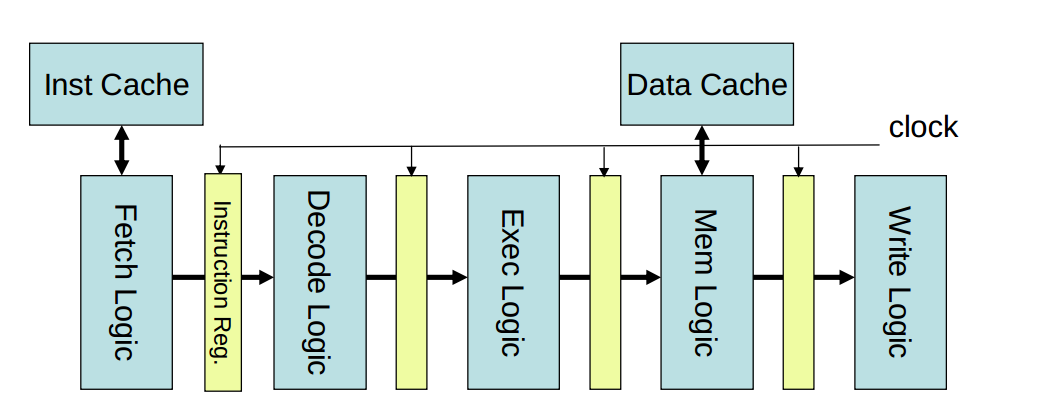
\includegraphics[width=\textwidth]{images/basic-pipeline}
  \caption{Using buffers between the different stages of the pipeline}
  \label{basic-pipeline}
\end{figure}

Now, we can still only execute one instruction per cycle, but we can also
increase our clock speed by five times, since each stage of the pipeline is
isolated by a buffer from the next!

\subsection{Control Transfer Problem}

Using a pipeline is fab if your instructions occur solely in a serial manner,
however, what if your program branches? The processor will only know that a
branch is happening at the \texttt{ID} stage of the pipeline, by which time
we've already fetched the next instruction!

If we come across a branch at the \texttt{ID} stage, then the fetched
instruction at the \texttt{IF} stage will have to be ignored all the way down
the pipeline, so we would waste one clock cycle (or more specifically, we would
waste $\frac{1}{5}$ of the work of five clock cycles!). The ignored instruction
is said to be a \textit{bubble} in the pipeline.

So far, we've assumed that our branch instruction has relies on no conditional
flags. If it did however, we would need to wait until the \texttt{EX} stage of
the pipeline before we knew what the outcome of the conditional evaluation would
be. This has the potential to create two bubbles, since if the branch was to
occur, the instructions at both the \texttt{IF} and \texttt{ID} stages of the
pipeline would have to be ignored.

These bubbles are called \textbf{control hazards}, and they occur when it takes
one or more pipeline stages to detect a branch. Longer pipelines are more likely
to suffer from control hazards more, since more of their pipeline will have been
processed by the time an instruction is detected to be a branch.

\subsubsection{Branch Prediction}

The main technique used to mitigate control hazards is \textbf{branch
prediction}. If we can remember what address a branch directed us to fetch next
from what it did when we executed that branch previously, then we could pre-
emptively load that instruction in the \texttt{IF} stage instead of fetching the
instruction at the PC.

In order to do this, we use a \textbf{branch target buffer}. This maps the
virtual address of one branch instruction onto the virtual address of the
instruction that is branched to, for example:

\begin{table}[ht]
  \centering
  \begin{tabular}{|c|c|}
    \hline
    \textbf{Branch instruction address} & \textbf{Next instruction address} \\ \hline
    \texttt{0xd4f30d2C} & \texttt{0xd4f30d60} \\ \hline
    \texttt{0xd4f30d0f} & \texttt{0xd4f30ddd} \\ \hline
    \multicolumn{1}{c}{\vdots} & \multicolumn{1}{c}{\vdots\vspace{0.2em}}\\ \hline
    \texttt{0xd4f30c4f} & \texttt{0xd4f30d6c} \\ \hline
  \end{tabular}
  \caption{An abstraction of what the datastructure inside a Branch Target
  Buffer could be like}
\end{table}

Now, we will always get unconditional branches right (after we've done it for
the first time), and we will get branches that are part of loops (such as a
\texttt{for} or \texttt{while} loop) right most of the time. If we predict a
branch incorrectly, we just get a bubble like we would if we had no branch
prediction, so it's a win-win situation.

Branch prediction is easy to understand, but implementing it is expensive. In
practice branch predictors use history of each branch (maybe taking the mode of
the last five branches), and the context of the branch (i.e. how did we get to
this point) in order to make a more accurate prediction.

\begin{figure}[ht]
  \centering
  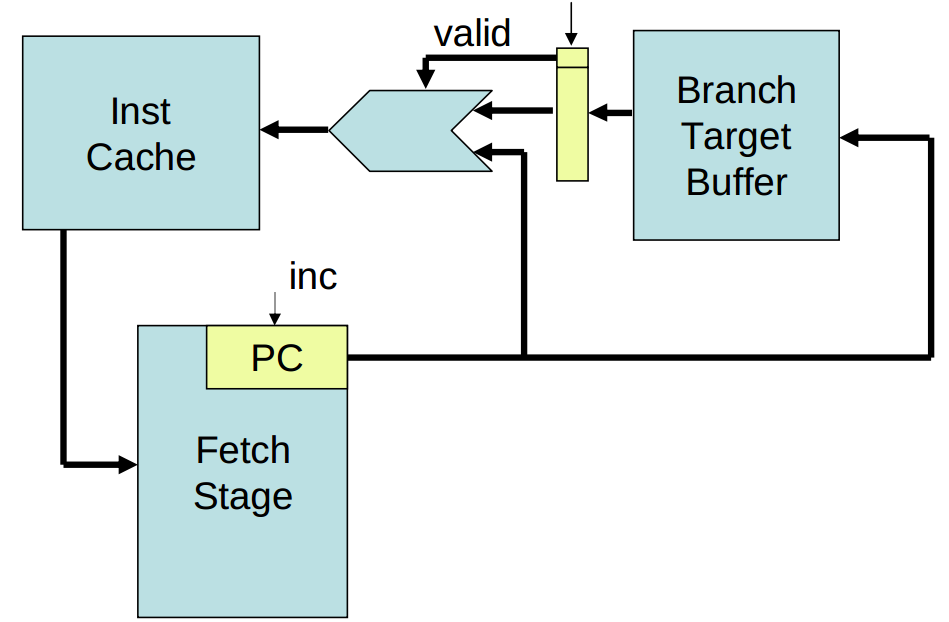
\includegraphics[width=0.5\textwidth]{images/branch-target-buffer}
  \caption{A BTB (Branch Target Buffer) in action}
  % TODO: Work out what this diagram is *actually* showing...
  \label{branch-target-buffer}
\end{figure}

\subsection{Data Hazards}

If we're using a pipeline to process instructions, then we have multiple
instructions at various stages of execution at the same time. This can cause
problems, if multiple instructions that are being executed in parallel operate
on the same resources. For example, if we execute the ARM Assembly code:

\begin{verbatim}
  ADD   R1, R2, R3
  MUL   R0, R1, R1
\end{verbatim}

\marginpar{This problem is called a `data not ready' issue.}

\marginpar{It might take two cycles for a value to be written into a register,
one for \texttt{EX} to complete and push the value into the register bank, and
another for the value to be written into the register.}

Here, the value in \texttt{R0} depends on that of \texttt{R1}. This is a
problem, because we only know the value of \texttt{R1} once the \texttt{ADD}
instruction has finished the \texttt{EX} stage, and the \texttt{MUL} instruction
will get the values from the registers while this is happening in it's
\texttt{ID} stage, henceforth we won't read the correct value of \texttt{R1}.

Two easy solutions to this problem are to:

\begin{itemize}
  \item Detect inter-instruction dependencies in hardware and withhold
  instructions in the decode stage until the data is ready. This creates the
  bubbles that we've worked so hard to avoid with branch prediction though!

  \item Have a compiler detect the dependencies, and have it re-order
  instructions to eliminate them. This is hard to do though, and often results
  in compilers inserting \texttt{NOP} (no operation) instructions that do
  nothing. These act like bubbles anyway, so we don't gain anything here either.
\end{itemize}

Since these are unsatisfactory, we could add extra paths to the pipeline between
the ALU output and the ALU input. They could be activated if there is an
interdependency so that the incorrect result of the \texttt{ID} stage could be
modified before being processed by the ALU.

\begin{figure}[ht]
  \centering
  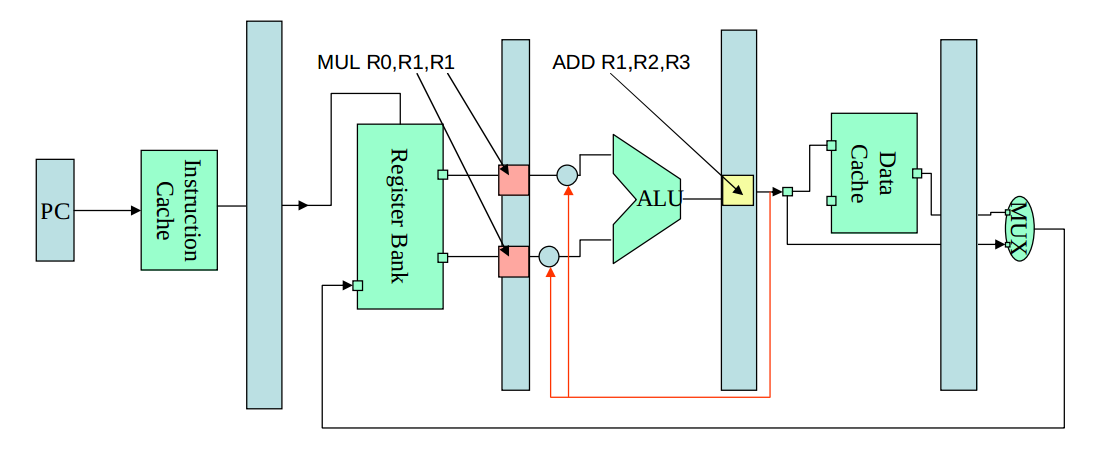
\includegraphics[width=\textwidth]{images/extra-paths}
  \caption{Here, we insert extra paths into the processor so that it can
  mitigate the \texttt{ADD}/\texttt{MUL} dependency.}
  \label{extra-paths}
\end{figure}

What if there is an interdependency with an instruction that might take a while
to execute, such as a memory read (\texttt{LDR})? If we have a program that
does:

\begin{verbatim}
  LDR   R1, [R2, R3]
  MUL   R0, R1, R1
\end{verbatim}

Our path would have to look like this:

\begin{figure}[ht]
  \centering
  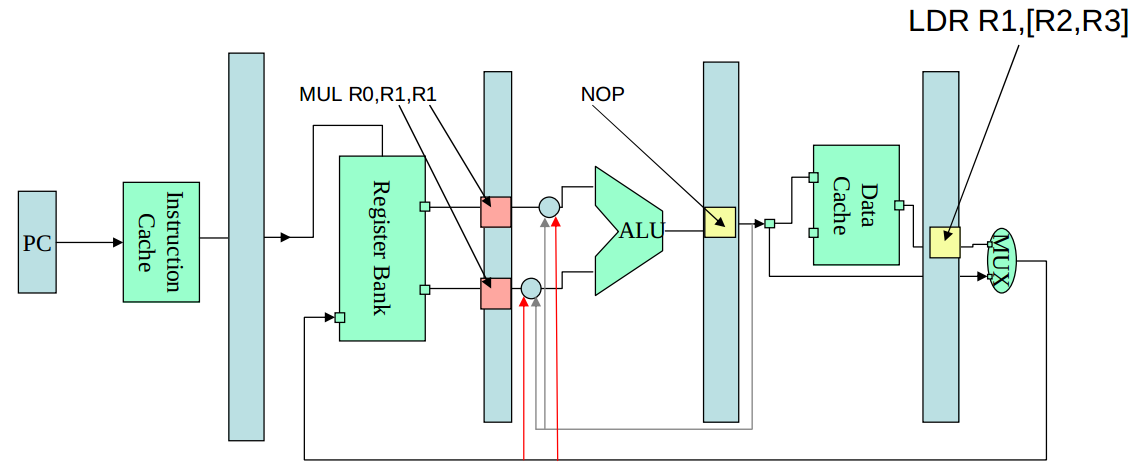
\includegraphics[width=\textwidth]{images/more-extra-paths}
  \caption{In order to cater for the worst case, where we're waiting on a memory
  read, we need even more extra paths.}
  \label{more-extra-paths}
\end{figure}

We want longer pipelines, since we want each stage of the pipeline to do as
little work as possible, taking as little time as possible, so that we can
increase the clock speed. However, as we do that, we will come across more
hazards, and we'll need to put more control paths in to mitigate them.
Eventually, there will come a point where increasing the length of the pipeline
will result in negative returns.

\subsection{Instruction Level Parallelism}

If there are instructions that do not depend on each other at all, for example:

\begin{verbatim}
  ADD   R0, R2, R3
  SUB   R1, R4, R5
\end{verbatim}

Then we could run these instructions at the same time, and not experience any
side effects. We may run into problems, if there are instructions that depend on
these two instructions having completed before they themselves execute, for
example:

\begin{verbatim}
  ADD   R0, R2, R3
  SUB   R1, R4, R5
  MUL   R0, R0, R1
  STR   R0, x
\end{verbatim}

We can draw a data flow graph to visualise these dependencies, and easily see
which instructions can be run in parallel:

\begin{figure}[ht]
  \centering
  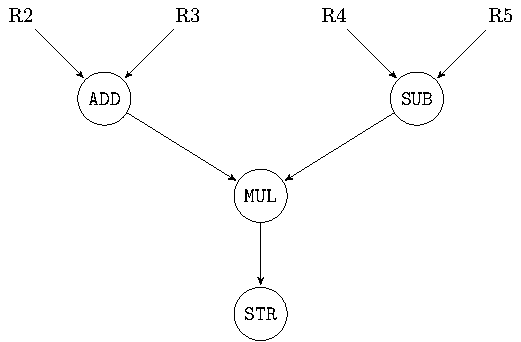
\includegraphics{diagrams/data-flow.pdf}
  \caption{A sample data flow graph.}
  \label{data-flow}
\end{figure}

Though this is a simple example, analysis has shown that it is not uncommon for
real programs to have up to four instructions that can be parallelised at some
point in the program's running time. Obviously, the amount of times when two or
three instructions could be parallelised will be greater than that of four.

In order to exploit this parallelism, we can:

\begin{itemize}
  \item Fetch multiple (in our case two for simplicity) instructions per cycle.
  \item Have multiple ALU's to execute instructions in parallel.
  \item Have common registers and caches, since the instructions are operating
  on the same data.
\end{itemize}

Now we could have an architecture looking like that in Figure~\ref{superscalar}.

\begin{figure}[ht]
  \centering
  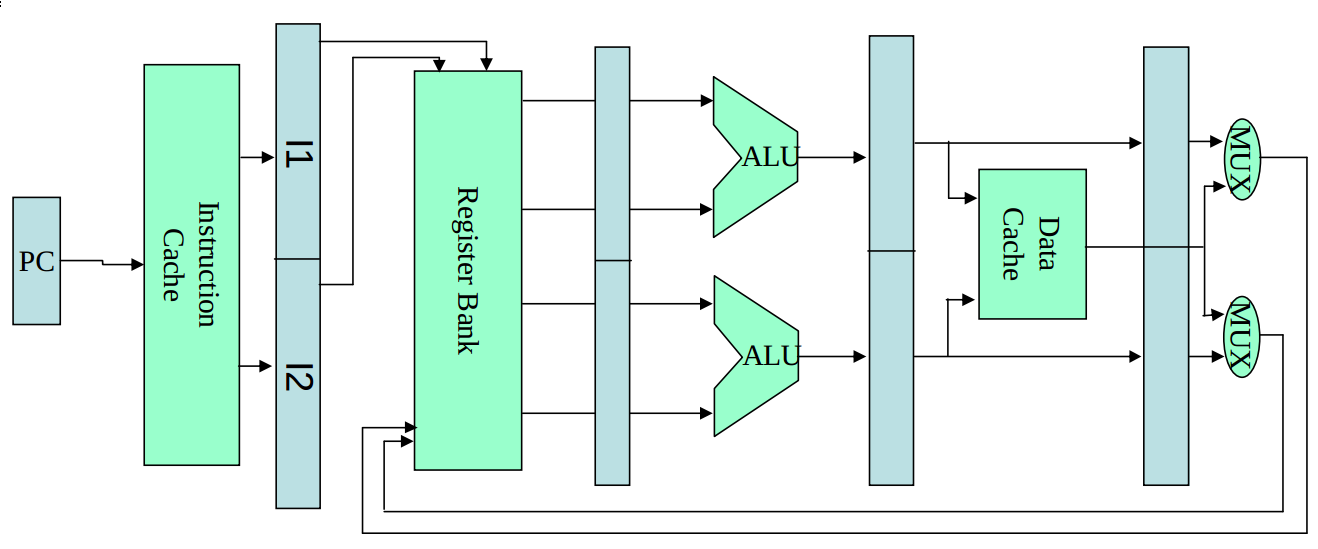
\includegraphics[width=\textwidth]{images/superscalar}
  \caption{A simple superscalar (implementing ILP) architecture.}
  \label{superscalar}
\end{figure}

\marginpar{Note, these multiple reads and writes will be occurring in different
parts of the register bank and cache, since the parallel instructions are (by
nature) independent of each other.}

If we are able to run multiple instructions at the same time, then our registers
and caches are going to have (in this case, which is a low level of parallelism)
roughly twice the load that they had previously. In order to allow them to handle
this extra load, we can make them \textbf{dual ported}, which means that the
access circuitry is duplicated so multiple reads and writes can happen
simultaneously.

In order to implement ILP, we also need a `dispatch unit' in hardware which is
part of the fetch stage (\texttt{IF}). This will fetch multiple instructions if
they are independent and be executed in parallel.

\subsubsection{Out of Order Execution}

In order to get the maximum number of ILP compatible instruction sequences in a
program, the compiler may be able to re-order instructions so that they have a
reduced number of interdependencies. One technique that is based on this is the
Very Long Instruction Word, where each word will be longer than a normal word
(maybe 48, 64 or more bits), and will contain more than one instruction.

Having the compiler re-order instructions means that it will sometimes add
\texttt{NOP}'s into the code, which can increase the binary size, and bloat the
code. The alternative it to rely on expensive hardware to detect out of order
opportunities at runtime.

To implement an out of order processor, you need to have a buffer that
instructions are fetched into, a scheduler to choose which (non-conflicting)
instructions to execute at what times, and a cache to store memory and register
accesses until all the instructions have finished so that the application can
execute normally as though all instructions executed in serial. Figure~\ref{out-
of-order} shows how this could all be implemented.

\begin{figure}[H]
  \centering
  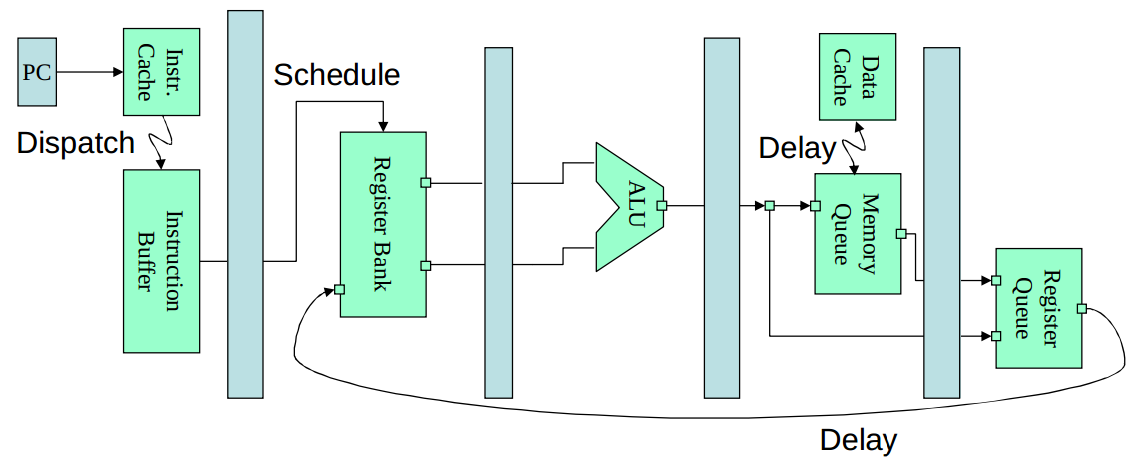
\includegraphics[width=\textwidth]{images/out-of-order}
  \caption{An example of how an out-of-order processor could be implemented.}
  \label{out-of-order}
\end{figure}

\subsubsection{Programmer assisted ILP}

Some processors now support SIMD (Single Instruction Multiple Data)
instructions, that allow one instruction to be executed on multiple
registers/memory locations etc. This is very useful when doing mathematical
computation with stuff like vectors and matrices, since it requires a lot of
repetitive operations that lend themselves easily to parallelism.

One example of this is the \texttt{UADD8} ARM instruction. It adds two registers
together into a third register like a normal add, but it does this four times;
once for each eight bit chunk in the registers. For example, \texttt{UADD8 R0,
R1, R2} will do:

\begin{figure}[H]
  \centering
  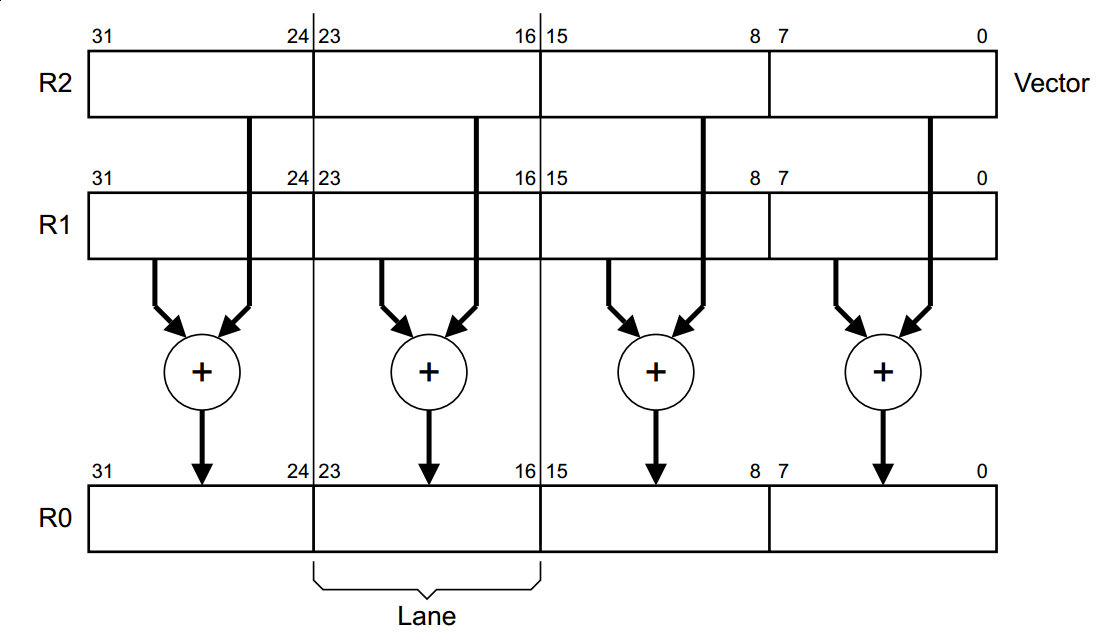
\includegraphics[width=\textwidth]{images/UADD8}
  \caption{A 4 way 8-bit integer add operation.}
  \label{UADD8}
\end{figure}

\section{Multi-Threading}

We have already seen, there are many different ways of increasing CPU
performance:

\begin{itemize}
  \item Increasing the clock frequency
  \item Increasing the \textit{ips} (instructions per clock)
  \item Minimising the impact of accessing memory with a cache
  \item Minimising bubbles (branch prediction)
  \item Minimising bubbles (out of order execution)
  \item Parallelising instructions (with an superscalar architecture)
  \item[ ] \hspace{-2.2em}And, up to a point
  \item Lengthening the pipeline
\end{itemize}

We have said that increasing the parallelism will speed up our pipeline, but in
order to do this, we need to find enough instructions to safely parallelise at
once. There are multiple ways to do this too:

\begin{itemize}
  \item When we get a branch instruction, do we pause until we evaluate the
  outcome of the branch, or keep issuing instructions? If we're using branch
  prediction, then we can keep issuing instructions.

  \item After a cache miss, we need to wait for a certain amount of time for the
  data we want to come from the memory, over the bus and into the CPU. While
  we're waiting, can we carry on issuing other instructions?

  \item Process instructions in parallel (e.g. with a superscalar architecture).

  \item Write to registers while the previous write is pending?
\end{itemize}

These ways of increasing parallelism are good, but assume we have only one source
of instructions. However in reality, a CPU will be executing code from multiple
processes at once. What about if we run out of instructions to execute in one
program, we could just context switch to another!

\subsection{Context switch}

In a context switch, the Operating System must load/store a lot of data about
the switching processes:

\begin{mymulticols}
  \begin{itemize}
    \item Process ID
    \item Process state
    \item Program Counter
    \item Stack Pointer
    \item General registers
    \item Memory management information
    \item Open file list (and positions)
    \item Network connections
    \item CPU time used
    \item Parent process ID
  \end{itemize}
\end{mymulticols}

\subsection{Hardware multithreading}

We could have two PC's, two sets of registers (GPR's on the diagram), two
virtual address mappings etc, and have the CPU support multi threading naively.
This would require the OS to be able to handle multiple processors, since the
easiest way of making it work is to make the one processor core look like two
processor cores (since the inputs and outputs are effectively doubled). See
Figure~\ref{hardware-multithreading-comparison} for a comparison of the three
types.

\begin{figure}[H]
  \centering
  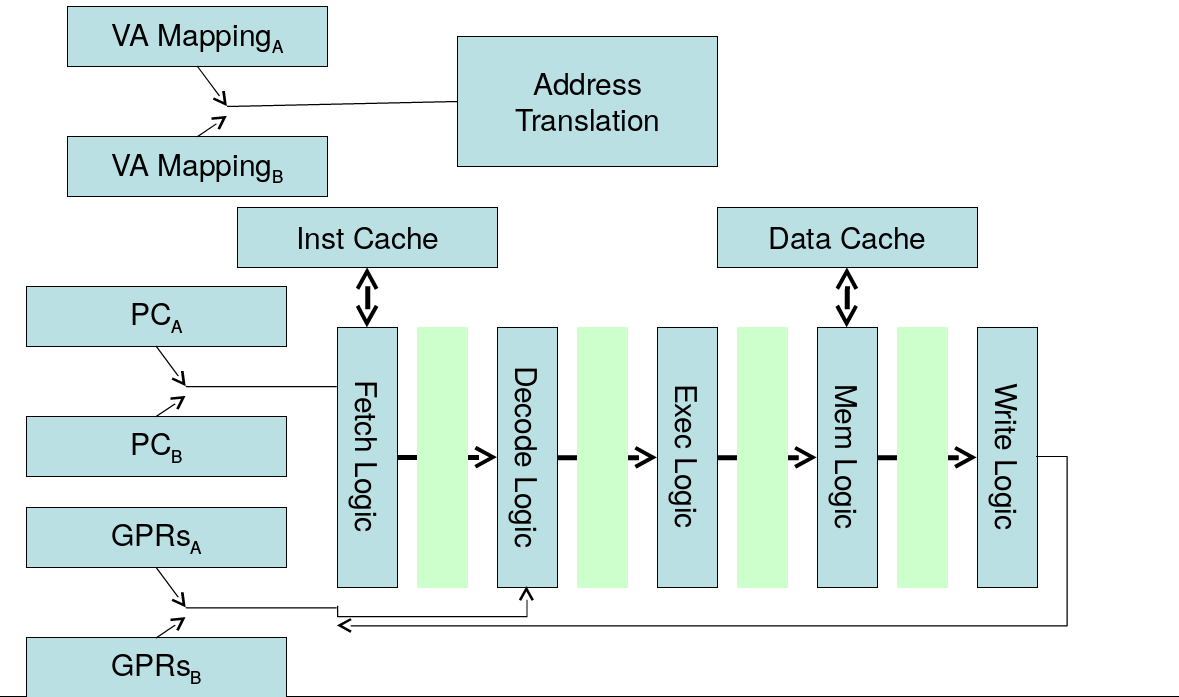
\includegraphics[width=\textwidth]{images/hyperthreading}
  \caption{The architecture of a multithreaded CPU}
  \label{hyperthreading}
\end{figure}

\begin{figure}[H]
  \centering
  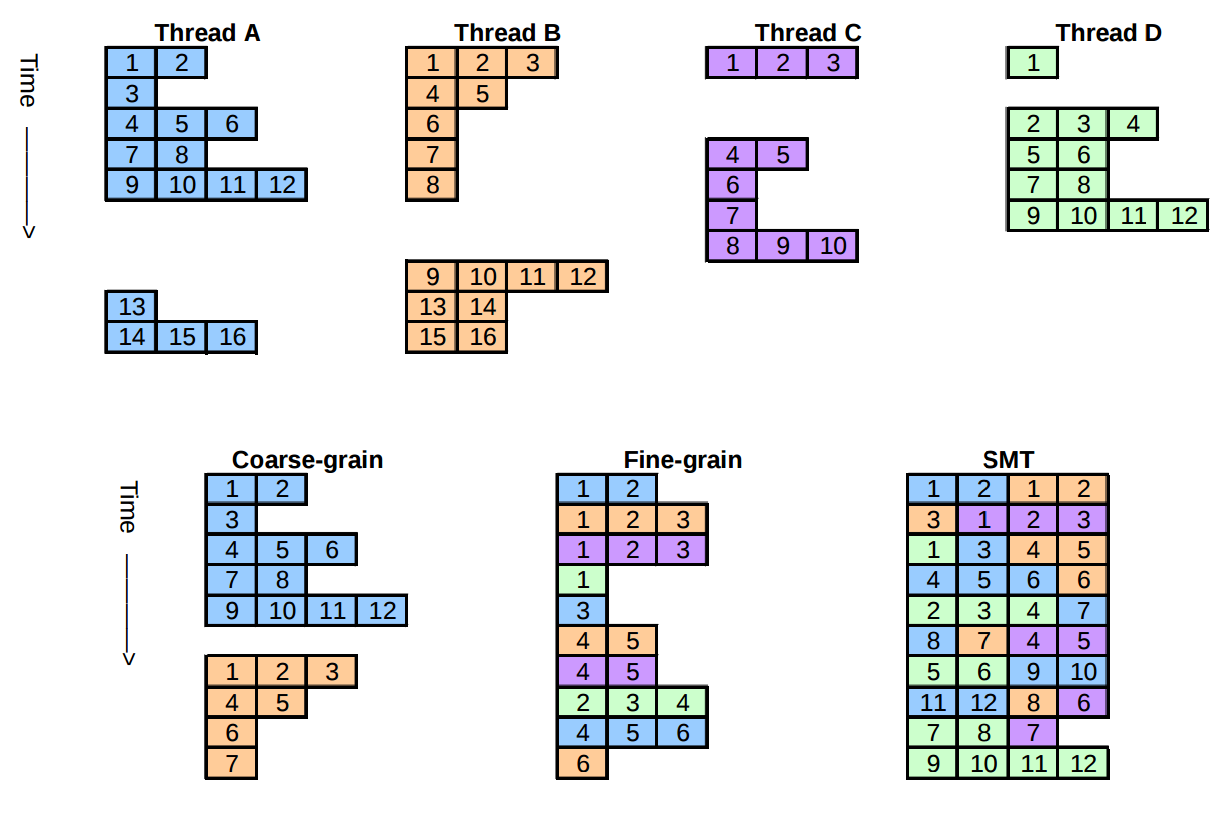
\includegraphics[width=\textwidth]{images/multithreading}
  \caption{How the three main types of hardware multithreading might execute
  simultaneous threads.}
  \label{hardware-multithreading-comparison}
\end{figure}

\subsubsection{Coarse grain multithreading}

Coarse grain multithreading is when you switch threads whenever the current
thread executes an expensive operation. This could be when there is a cache miss
for example, or whenever the CPU has to wait to execute more instructions.

This type of multithreading has benefits. If the CPU can execute one instruction
per nanosecond ($1GHz$), a cache miss takes $20$ nano seconds, and one cache
miss occurs on average, every hundred instructions, then the time number of
instructions per clock cycle is:

\begin{description}
  \item \textbf{Without multithreading}
    \[
      \frac{100ns}{100ns + 20ns \text{(one hundred instructions and one cache miss)}} = 0.8333
    \]
  \item \textbf{With multithreading}
    \[
      \frac{100ns}{100ns + 1ns \text{(one hundred instructions and context switch)}} = 0.99
    \]
\end{description}

Coarse grain multithreading is good, because it requires a minimal change in the
pipeline; only to abort instructions in the `shadow' of a cache miss and the
ability to resume the instruction stream at the correct point afterwards.

%Unfortunately, when you do a context switch, a new program runs on the
%processor. This is bad, since both the instruction and data caches will suddenly
%contain an awful lot of entries that are obselete, and so most of the cache
%requests will be misses.

\subsubsection{Fine grain multithreading}

The aim of fine grain multithreading is to be able to switch between CPU threads
with as little overhead as possible. This involves interleaving the instructions
of several threads. This results in better overall performance, since the impact
of short stalls such as accessing memory or the cache is alleviated by executing
instructions from other threads. Each individual thread perceives it is being
executed slower, but the overall performance is better.

\subsubsection{Simultaneous multithreading (SMT)}

The idea behind SMT is to exploit both instruction level parallelism and thread
level parallelism at the same time. In a superscalar processor (i.e. one that
can execute more than one instruction per clock cycle), we can issue
instructions from different threads in the same cycle.

SMT requires a significant overhead, and is only really feasible to processors
with an out of order execution capability.

\subsubsection{Disadvantages of hardware multithreading}

Threads can `trash' the cache for other threads, since they will probably have
completely different access patterns, so the overall cache performance may
decrease. This will not occur if different threads are accessing the same areas
of memory, but this is a relatively rare case (since processes can only access
disjoint areas of memory) unless a process has multiple threads processing.

Furthermore, there is a significant increase in the complexity of the hardware
required. The thread state, priorities, OS-level information etc must all be
maintained by the processor in hardware.

\subsubsection{Other techniques}

\begin{description}
  \item \textbf{Slipstreaming}:\\
    This is when an application is split into two parts; the critical path, and
    all the rest. The critical path will run ahead, and pass the result of the
    operations back to the `main thread'
  \item \textbf{Memory prefetching}:\\
    We could compile the application into two parts here too, except one will
    get all the memory accesses, and the other will do everything else. This
    means that the data will always be in the cache when it is needed in the 
    second thread.
  \item \textbf{Speculative execution}:\\
    When we get to a conditional branch in the program, we could spawn two
    threads; one for each path. When we know which is the correct path, we can 
    kill the thread that wasn't executing that path. In this way, we could avoid
    control hazards.
\end{description}

\section{Multi-Core}

Since Moore's law is slowly coming to an end, chip designers are having to look
to other techniques to increase performance. Cooling is a serious problem now,
since there are so many transistors on chips, that the power density (watts per
unit area) is becoming unsustainable. Smaller transistors have very
unpredictable characteristics, and the architecture of processors is becoming so
complex that it's hard to reason about.

Older problems are becoming worse too; memory is still not getting faster at the
same rate as processors are, and as a result even when the clock speed and the
instructions per second increases on the processor, lots of the time it may be
sat idle.

Lots of solutions have been tried and implemented to increase single core
performance:

\begin{mymulticols}
  \begin{itemize}
    \item Caching
    \item Pipelines
    \item Superscalar processors
    %TODO: Ummm?
    \item Out of order processing
    \item Multithreading
    \item Branch prediction
    %TODO: Ummm?
    \item Forwarding
    %TODO: Ummm?
    \item Register renaming
  \end{itemize}
\end{mymulticols}

However, these all have a limited scalability; the hardware costs increase in a
roughly quadratic manner but the performance increase is sublinear.

Another way to speed up execution is to have multiple CPU cores on one chip.
Multiple simple cores may achieve a higher performance than one complex core
whilst being easier to design.

There are different opinions on how to connect the processors; should they all
access the same memory, or each have their own? From a software point of view,
it is easier to have processors that can access shared memory (since
synchronization is implicit) than having separate memories. Unfortunately,
after a few cores, shared memory becomes harder to attain.

Having more cores does not speed up programs without the programs making use of
the cores explicitly. Threads must be spawned by a program if it wants to
execute on more than one core, however, different programs can run concurrently
on different cores. For example, one core could run an antivirus scan, while
another could run a web browser.

\subsection{The structure of a multi core processor}

In a multicore processor, some components will be shared between processors, and
some won't. Usually, each processor shares an L1 cache, and sometimes an L2
cache. You can see a generalisation in Figure~\ref{multicore-arch}.

\begin{figure}
  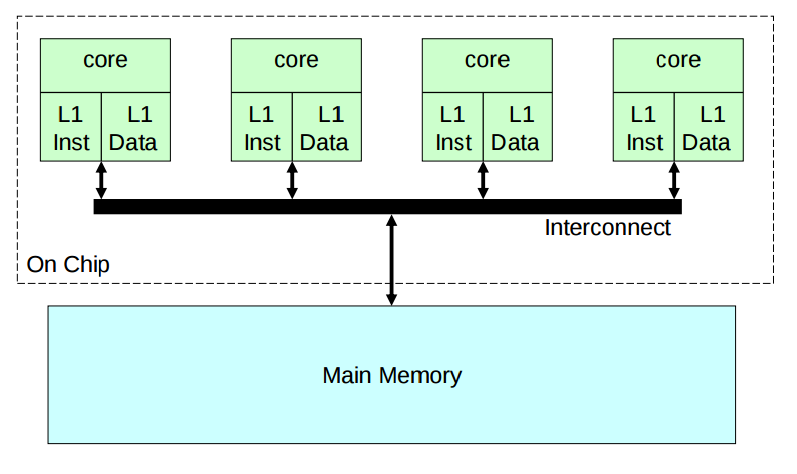
\includegraphics[width=\textwidth]{images/multicore-arch}
  \caption{A simplified multicore architecture}
  \label{multicore-arch}
\end{figure}

\subsection{Data coherency and consistency}

Different CPU cores trying to access the same areas of memory can be an issue,
since the caches may not be \textit{coherent}. Coherence is a desired property
of multiple caches all pointing to the same shared resource; each cache should
provide the same view of the resource at all times (from the point of view of
the users of the cache).

This shouldn't be a problem, since after all, processes have disjoint memory
spaces, so each process will be running on one core and accessing different
areas of memory. However, threads \textit{do} share memory, and they can run on
multiple cores (and other stuff can update memory, such as DMA etc).

When we talk about CPU cache coherency, the L1 cache is what we mainly focus on.
Each core will have its own L1 cache, and if a value is updated in one cache
that the others are also holding, then the other caches will be immediately out
of date. Even if we wrote back to memory on every cache write, the other cores'
caches wouldn't be updated. We need to ensure that every core has an up-to-date
cache at all times.

\marginpar{You can think of consistency as representing the model of the
machine as presented to the programmer. If one thread updates a value in memory,
it is expected that all the other threads will also be able to see that update.}

Sometimes, we want to read and update a memory location as a single atomic
operation, and make sure that no other threads can update the same location at
the same time.

\textbf{Sequential consistency} is the idea that memory operations should appear
to execute one at a time, even though they may not do in practice. Leslie
Lamport describes it as:

\begin{aquote}{Leslie Lamport}
  The result of any execution is the same as if the operations of all the
  processors were executed in some sequential order, and the operations of each
  individual processor appear in this sequence in the order specified by its
  program.
\end{aquote}

Since lower down the technology stack of a running program, instructions may be
executed out of order (for example in Java), the compiler must insert special
instructions such as the following to ensure that consistency is maintained:

\begin{description}
  \item \textbf{Fence}:\\
    A fence will make sure each memory access before the fence completes before
    new ones are started.
  \item \textbf{Barrier}:\\
    All threads in the program must reach the barrier before any of them can
    continue executing.
  \item \textbf{Lock}:\\
    Only one thread can enter a section of the program that is protected by a 
    lock at any one time. That section may be referred to as atomic.

    Hardware support is usually required to implement locks, since normal memory
    reads and writes cannot be guaranteed to be atomic without, guess what\dots
    locks!
\end{description}

There is some Instruction Set Architecture support for synchronization, such as
atomic `compare and swap' instructions conditional load and stores (based on if
the memory location has mutated since it was last accessed), and transactional
memory.

\textbf{Transactional memory} allows you to read and write to memory with no
restrictions, however once the operation is completed, the transaction is
checked to see if it conflicted with any other transaction, and it is rolled
back if it did (and started again).

\subsubsection{Coherence protocols}

A scheme where each core would what other cores are caching the same data as it
is would be far too complex. As an alternative to this, each cache
\textit{snoops} on the other caches for activity related to its own cache. This
is most simply implemented by routing all data through a bus so every cache can
see the activity of other caches.

There are two very simple snooping protocols in use:

\begin{description}
  \item \textbf{Write Update}:\\
    When a core writes a value to memory, it is updated in its local cache. The
    cache then broadcasts the address and new data to the bus and all the
    snooping caches update their own copy.
  \item \textbf{Write Invalidate}:\\
    A core that wants to write to an address writes to its own cached copy, but
    also sends a `write invalidate' message that will tell the other cores
    to invalidate the cache line that they have stored. Any read to that address
    will now miss.
\end{description}

In both schemes, the bus makes sure that only one core can use the bus at one
time, so that simultaneous writes do not occur. Though the first option (write
update) might look fastest, it isn't always, since it will update the cache when
it might not be needed (e.g. two writes to the same cache in a row would require
two updates to the other caches, but only one invalidate using write
invalidate). This can also happen when you're writing to different words in the
same block of a multi word cache.

Unfortunately, this can happen often due to spatial and temporal locality (the
principles that make CPU caches work), and bus bandwidth is a precious
commodity, especially in shared memory multi-core chips. Invalidate protocols
have been modelled to use less bandwidth, and so these are more commonly used.

In both of the above schemes, merely knowing if other CPU caches hold the value
is enough to know whether to send a message on the bus in the first place.

If we use the invalidation scheme, then if the writes don't also get written
through to memory, then when other caches read from the memory, they will read
old values, so we need a protocol to handle this.

\textbf{MESI Protocol}

This is a practical multi-core invalidation protocol which tries to minimise the
bus usage. It also implements a `copy back' scheme where the main memory or L2
cache is not updated until a `dirty' cache line is displaced. 

As a result of this, cache lines have two state bits, meaning they can be in the
following states:

\begin{description}
  \item \textbf{Modified}:\\
    The cache line has been modified and is different from the main memory (i.e.
    it's a dirty copy).
  \item \textbf{Exclusive}:\\
    The cache line is exactly the same as main memory and it's the only copy.
  \item \textbf{Shared}:\\
    It's the same value as the main memory, but other copies may be in other
    caches which may differ.
  \item \textbf{Invalid}:\\
    The cache line data is not valid.
\end{description} 

Another protocol called \texttt{MOESI} has another state:

\begin{description}
  \item \textbf{Owned}:\\
    The cache line has been modified and is different from memory. There are
    other copies in other caches.
\end{description}

\marginpar{Owned means that we don't have to copy back to main memory on writes.
}

The changes of state of the cache line are dependent on the memory access
events, which can be either from local core activity or snooping from other
cores. The cache line state will only be effective if its address matches the
address of the memory event.

The state changes are as follows:

\begin{figure}[H]
  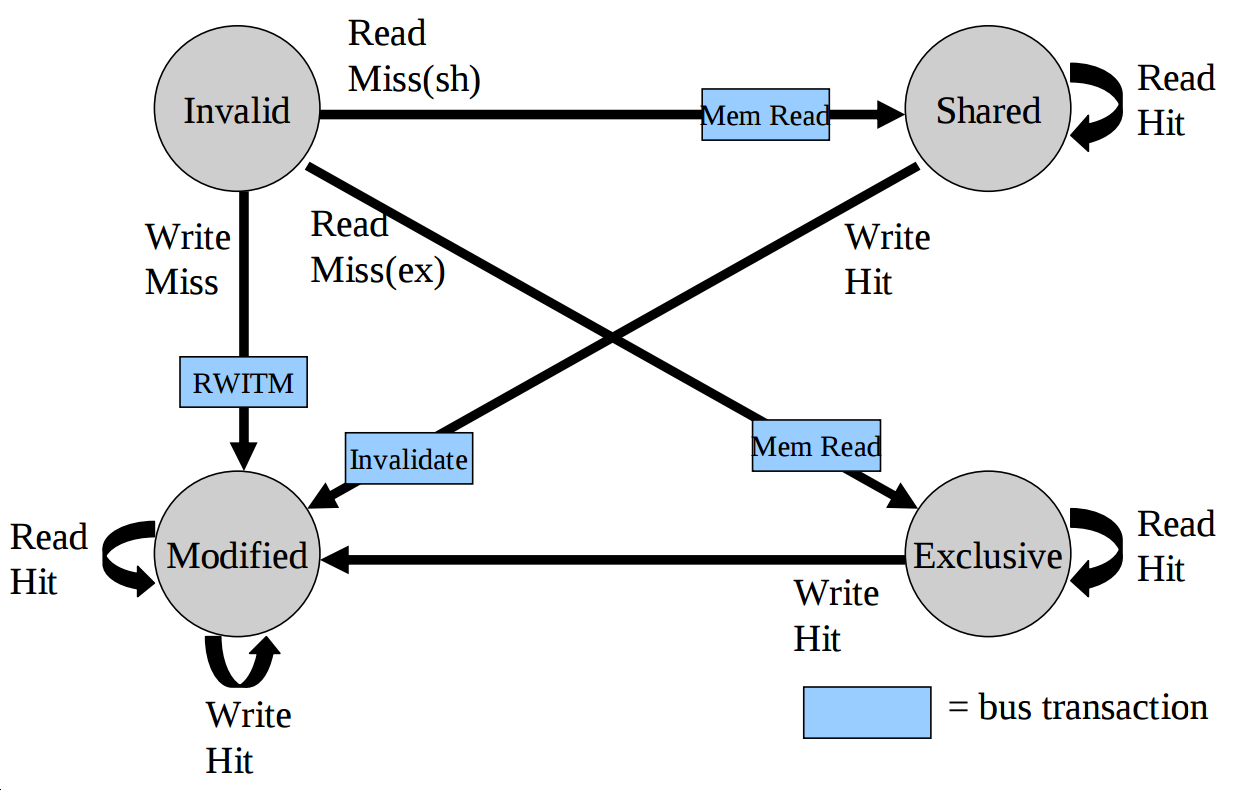
\includegraphics[width=\textwidth]{images/MESI1}
  \caption{MESI - local cache view}
  \label{MESI1}
\end{figure}

\marginpar{`RWITM' means Read With Intent To Modify.}

\begin{figure}[H]
  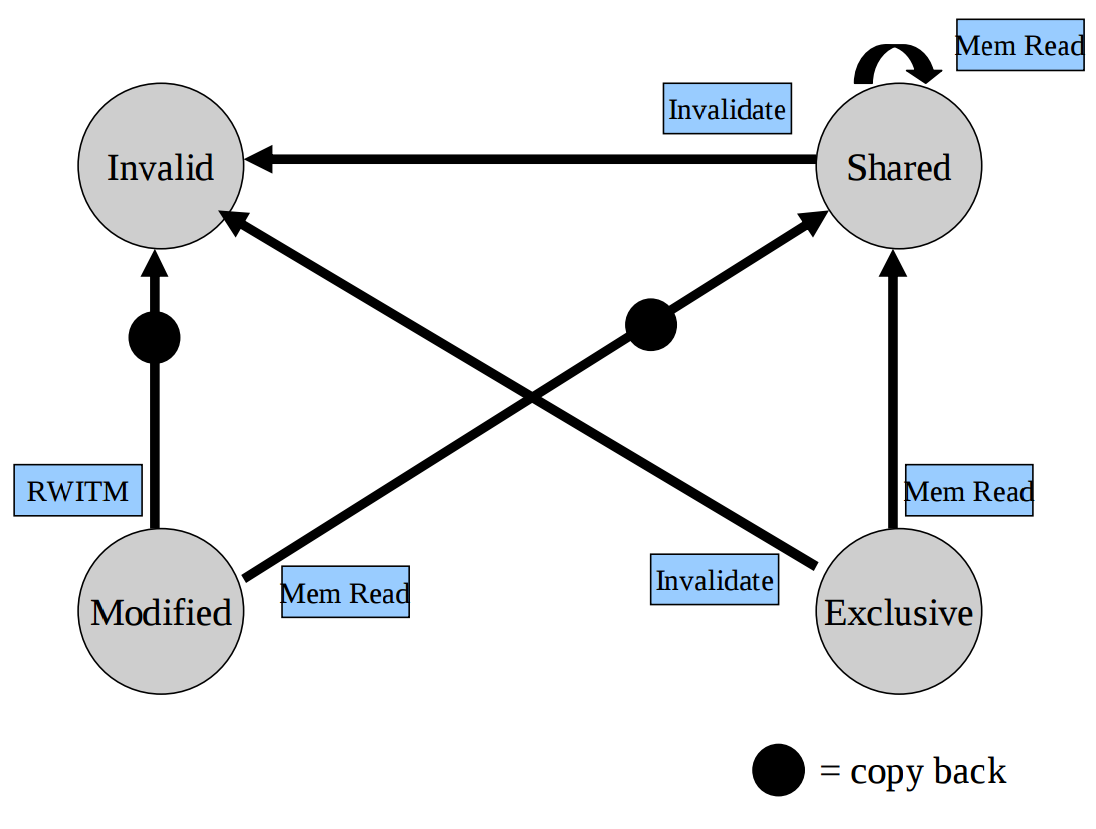
\includegraphics[width=\textwidth]{images/MESI2}
  \caption{MESI - snooping cache view}
  \label{MESI2}
\end{figure}

The consensus is that snooping protocols don't scale well beyond around 16 cores
max, since the bus connecting the cores becomes saturated. We could have a
hierarchy of buses, but this is complicated.

Instead, we can create directory based protocols. If we use distributed
hardware, we can have a directory listing what data other caches have, and
caches can talk to each other in a point-to-point manner. Since there is more
traffic required for this between the cores, the bus is often replaced with a
network on a chip.

The cache lines can be in three states that are like those of MESI:

\begin{itemize}
  \item \textit{Invalid}
  \item \textit{Shared} (coherent with the main memory)
  \item \textit{Modified} (value is changed and no other copies are anywhere)
\end{itemize}

The directory can have three states too:

\begin{itemize}
  \item \textit{NC} (Not Cached; the cache line isn't present anywhere)
  \item \textit{Shared} (the cache line is present in at least one core)
  \item \textit{Modified} (the cache line is modified and is in one other core)
\end{itemize}

The directory also stores a \textit{sharing vector} describing what core holds
the same cache line, which can be seen in Figure~\ref{directory-protocol}.

\begin{figure}[H]
  \centering
  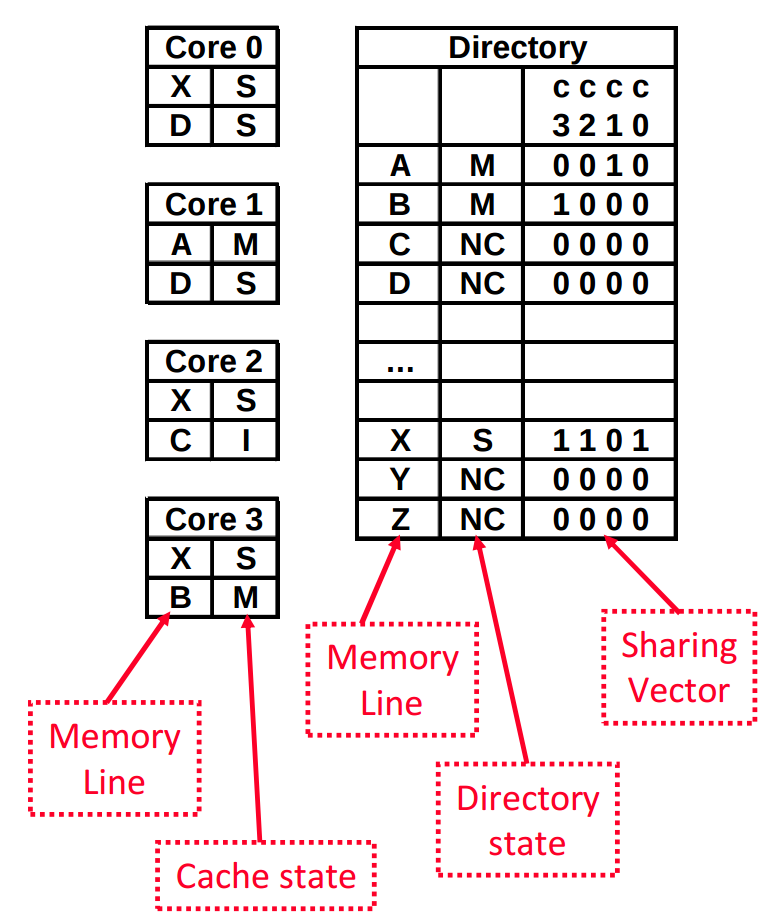
\includegraphics[width=0.5\textwidth]{images/directory-protocol}
  \label{directory-protocol}
  \caption{How data might be organised in a directory protocol}
\end{figure}

If we have a central directory, then it might become the bottleneck we were
trying to avoid with a bus. To stop this, we could use a distributed directory,
where each core has its own directory, this requires an extra flag `home' which
indicates the data is stored locally.

To sum it up, directory protocols are:

\begin{itemize}
  \item More scalable (better for CPU's with more cores).
  \item Use p2p messaging to simplify interconnection and allow parallel
    communication.
  \item Each core doesn't have a global view of the caches, we need to store the
    state separately in the directory.
  \item Control is more complex, but performance is better overall.
\end{itemize} 

\subsection{On-chip interconnects}

So far, we've only really considered buses as a way of communicating between
cores, however we could use a network on a chip (NoC) to communicate. Things we
need to consider about networks on a chip are:

\begin{mymulticols}
  \begin{itemize}
    \item Bandwidth
    \item Latency
    \item Congestion
    \item Fault tolerance
    \item Area ($mm^2$)
    \item Power dissipation
  \end{itemize}
\end{mymulticols}

There are three important features of a NoC; topology (how the cores and network
infrastructure is organised), routing (how the traffic moves around) and
switching (how the traffic moves from once component to another).

The medium through which data is transmitted is a bus. Buses are single usage at
any one time and are controlled by a clock that divides its use into time slots.
Transactions are often split, since a message will be sent in one slot, and th
reply received in another later slot (slots can be used in between these two
events).

Networks on a chip can take many different forms though:

\begin{center}
  \begin{tabular}{| m{2cm} | m{5cm} | c |}
    \hline
    Crossbar & You can connect $n$ inputs to $n$ outputs & 
    \begin{minipage}{.3\textwidth}
      \begin{center}
        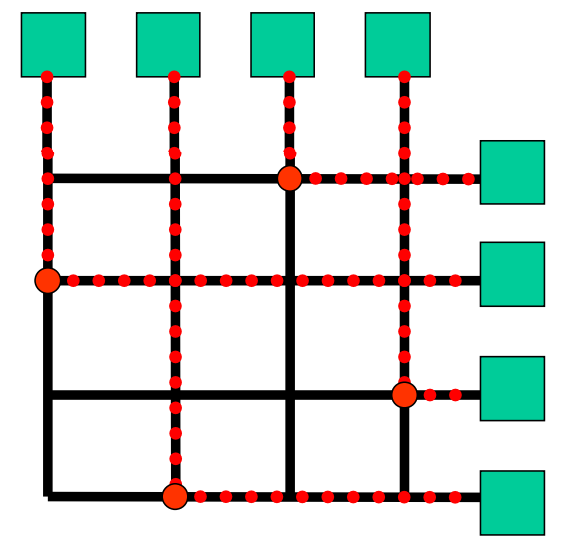
\includegraphics[width=0.5\linewidth]{images/crossbar}
      \end{center}
    \end{minipage} \\ \hline
    Ring & Simple, but low bandwidth and variable latency & 
    \begin{minipage}{.3\textwidth}
      \begin{center}
        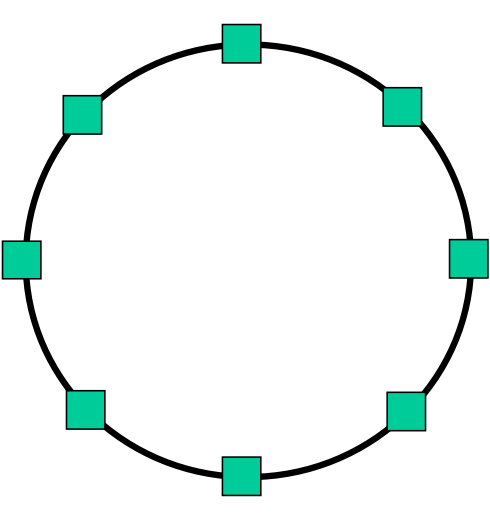
\includegraphics[width=0.5\linewidth]{images/ring}
      \end{center}
    \end{minipage} \\ \hline
    Tree & Variable bandwidth and latency (depth etc), may be unreliable & 
    \begin{minipage}{.3\textwidth}
      \begin{center}
        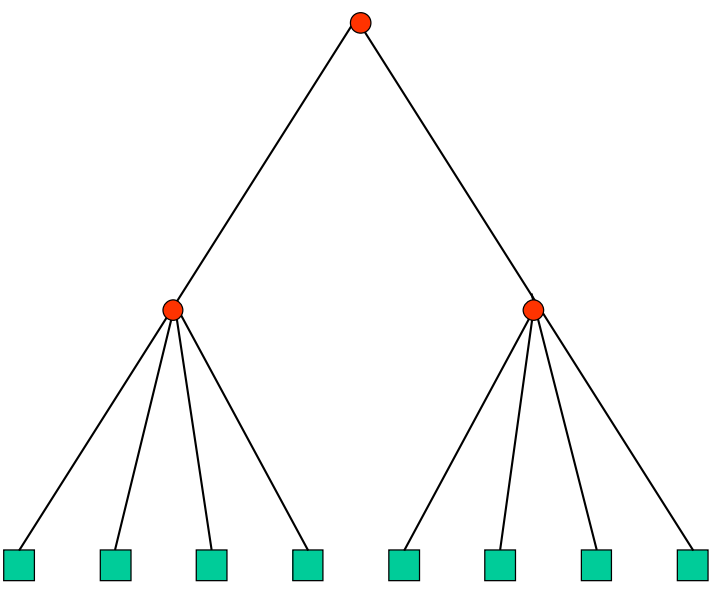
\includegraphics[width=0.5\linewidth]{images/tree}
      \end{center}
    \end{minipage} \\ \hline
    Fat tree & Faster, more reliable, but uses more resources than a tree & 
    \begin{minipage}{.3\textwidth}
      \begin{center}
        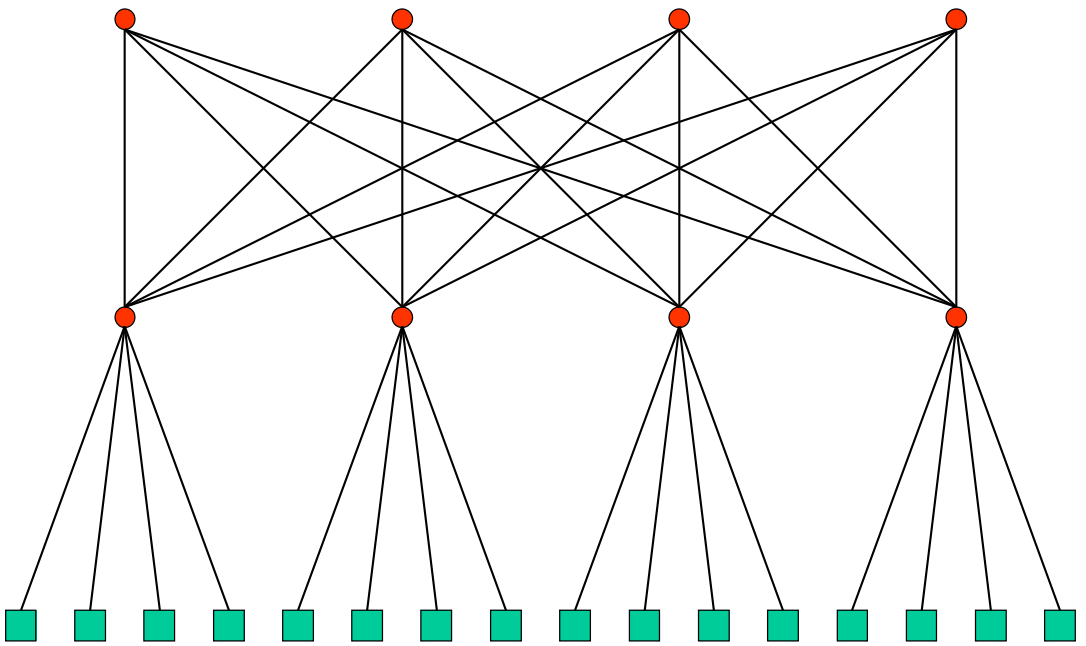
\includegraphics[width=0.5\linewidth]{images/fat-tree}
      \end{center}
    \end{minipage} \\ \hline
    Mesh & Okay bandwidth, variable latency, but good for large systems because
    of the layout & 
    \begin{minipage}{.3\textwidth}
      \begin{center}
        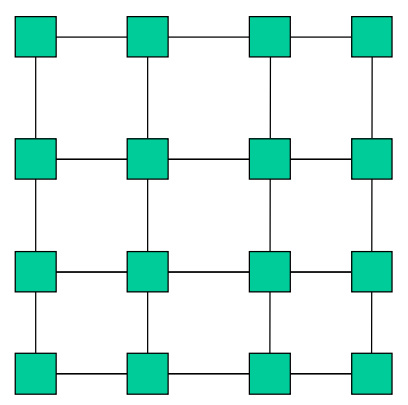
\includegraphics[width=0.5\linewidth]{images/mesh}
      \end{center}
    \end{minipage} \\ \hline
  \end{tabular}
\end{center}

\subsubsection{Routing}

There are three types of routing we're going to look at:

\begin{center}
  \begin{tabular}{| m{2cm} | m{5cm} | c |}
    \hline
    Minimal &
    \begin{itemize}
      \item Always selects the shortest path
      \item Packets move closer at every step
      \item But are more likely to be blocked
    \end{itemize} & 
    \begin{minipage}{.3\textwidth}
      \begin{center}
        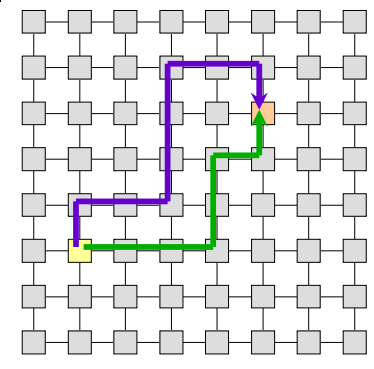
\includegraphics[width=0.5\linewidth]{images/minimal}
      \end{center}
    \end{minipage} \\ \hline
    Oblivious &
    \begin{itemize}
      \item Unaware of network state
      \item Packets take a fixed path
      \item Very simple and deadlock free
      \item Prone to contention
    \end{itemize} & 
    \begin{minipage}{.3\textwidth}
      \begin{center}
        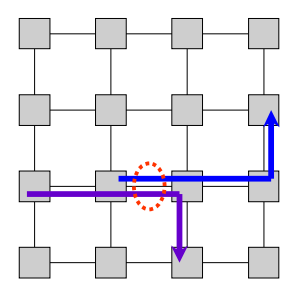
\includegraphics[width=0.5\linewidth]{images/oblivious}
      \end{center}
    \end{minipage} \\ \hline
    Adaptive & 
    \begin{itemize}
      \item Aware of network state (moves packets to avoid contention)
      \item Higher performance
      \item More area and power required
      \item Deadlock prone (more hardware needed)
      \item Rarely used in NoC's
    \end{itemize} & 
    \begin{minipage}{.3\textwidth}
      \begin{center}
        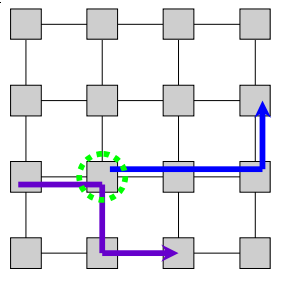
\includegraphics[width=0.5\linewidth]{images/adaptive}
      \end{center}
    \end{minipage} \\ \hline
  \end{tabular}
\end{center}

\subsubsection{Switching}

There are two types of packet switching we'll look at, store and forward and
wormhole switching. The premise is that data is split into small packets, some
extra information is added to enable them to get to their destination and they
are sent into the network. This allows time-multiplexing of network resources
and is good for performance (especially in short messages). Packets are also
split into flits, which are teeny packets (see Figure~\ref{flits}).

\begin{figure}
  \centering
  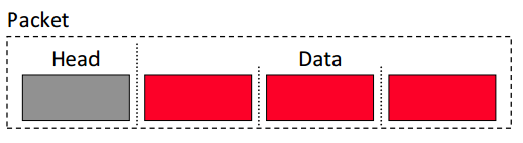
\includegraphics[width=0.5\linewidth]{images/flits}
  \caption{How a packet is split up into flits.}
  \label{flits}
\end{figure}

\begin{center}
  \begin{tabular}{| m{2cm} | m{5cm} | c |}
    \hline
    Store and forward &
    \begin{itemize}
      \item A packet is not forwarded until all its phits arrive to each node
      \item Failure detection happens on the fly
      \item But performance is low
      \item And large buffers are required
    \end{itemize} & 
    \begin{minipage}{.3\textwidth}
      \begin{center}
        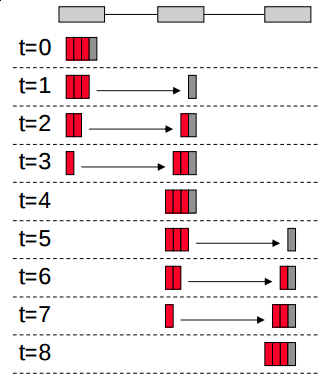
\includegraphics[width=0.5\linewidth]{images/store-and-forward}
      \end{center}
    \end{minipage} \\ \hline
    Wormhole &
    \begin{itemize}
      \item A packet is forward as soon as its head arrives
      \item Performance is better than store and forward
      \item But fault detection is only possible at the destination
      \item Less hardware
    \end{itemize} & 
    \begin{minipage}{.3\textwidth}
      \begin{center}
        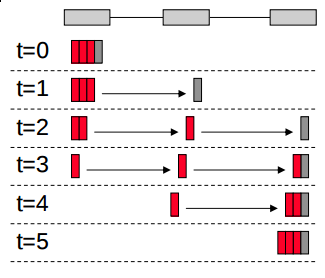
\includegraphics[width=0.5\linewidth]{images/wormhole}
      \end{center}
    \end{minipage} \\ \hline
  \end{tabular}
\end{center}

\section{Virtualization}

\begin{wrapfigure}{R}{0.3\textwidth}
  \centering
  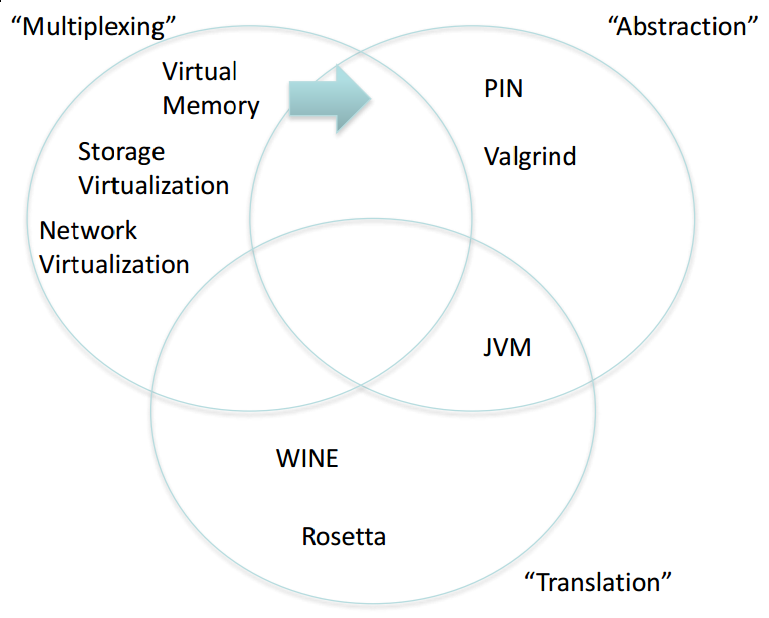
\includegraphics[width=0.25\textwidth]{images/types-of-virtualization}
  \caption{The different types of virtualization. PIN is a tool to annotate
  binary executables if you hadn't heard of it.}
  \label{types-of-virtualization}
\end{wrapfigure}

Virtualization isolates the details of the hardware from the software that uses
it. You can break virtualization down into two broad categories:

\begin{description}
  \item \textbf{Process Virtualization}:\\
    Run a process under the control layer of software. The JVM does this.
    \marginpar{Here, a ``layer of software'' can mean a lot of things, but
    generally one or more processes.}
  \item \textbf{System Virtualization}:\\
    Run a whole OS under the control of a layer of software, e.g. VMware.
\end{description}


This is useful, since virtualization can translate between technologies
(different instruction sets, system calls etc), change the level of abstraction
(providing garbage collection, debugging etc) and even make the system resources
look different (emulate CD drives, reduce the amount of RAM for a virtual
machine).

For example, the JVM interprets byte code, and maps it onto the host OS's API.
Rosetta translates PowerPC binaries to x86 ones on the fly.

\subsection{The details of virtualization}

A virtualised OS runs on top of a Virtual Machine Monitor (VMM) or Hypervisor.
This often (but not always, since it is sometimes one itself) sits on top of the
\textit{actual} operating system running on the machine. The VMM will handle
physical resource access for the guest OS since it runs in a privileged mode,
and it makes sure the guest OS is isolated from other resources. These resources
include:

\begin{mymulticols}
  \begin{itemize}
    \item Timers
    \item CPU registers
    \item CPU flags (e.g. interrupt enable)
    \item Device control registers (DMA, interrupt IO etc)
    \item Memory mapping (page table etc)
  \end{itemize}
\end{mymulticols}

Often, when a guest OS tries to access resources its not allowed to, it will
trigger a trap instruction on the VMM, which allows the VMM to check the bounds
of access for that instruction/OS and proceed accordingly. Since the VMM does
the privileged operations, the guest OS can be unprivileged.

This can be tricky sometimes though; some instructions behave differently
according to what mode they are in, so the VMM must learn to handle that.

If the guest OS is virtualization aware, then it is much easier to build a VMM,
since the guest OS can call the VMM specifically for privileged operations,
cooperate with the VMM over shared page tables and call the VMM for IO.

\subsection{Operations on VM's}

When you start a VM, the hypervisor will save the current registers, load the
VM's initial registers and jump to the new VM's PC address. Likewise, when a VM
is stopped, the hypervisor will save its registers into its own memory space. It
is important to not that VM's are stopped and started all the time so that the
CPU (and other resources) can be shared.

When the VM is stopped, its memory and IO state is also retained as well as its
CPU registers. It is best to stop a VM when its IO is \marginpar{Quiescent means
to be `in a state or period of inactivity or dormancy'}\textit{quiescent}, so
that we don't have to save loads of IO buffers etc.

Once we've stopped a VM, we can freeze it by saving all this state into a file.
This file tends to be large, since it contains the whole operating system, its
installed applications and the state such as the registers etc.

Because virtual machines can be stored as files, there are a number of things we
could do with them:

\begin{mymulticols}
  \begin{itemize}
    \item Move a VM onto a different machine
    \item Snapshot the state of a VM and roll it back later
    \item Archive a VM into a database or secondary storage
    \item Quickly start an archived VM (rapid provisioning)
    \item Live migration (we'll get on to this)
    \item Load balancing (and this)
  \end{itemize}
\end{mymulticols}

\subsubsection{Live migration}

Wouldn't it be good to be able to move a VM from one machine to another without
pausing execution of the VM? That means we could change the physical machine a
VM is running on (maybe to repair or upgrade the old one) with minimal
interruption for the end user.

I'm going to use Wikipedia's explanation for this, since it's really good:

\begin{aquote}{\url{http://en.wikipedia.org/wiki/Live_migration}}
  \textbf{Warm-up phase}
  
  In pre-copy memory migration, the Hypervisor typically copies all the memory
  pages from source to destination while the VM is still running on the source.
  If some memory pages change (become `dirty') during this process, they will be
  re-copied until the rate of re-copied pages is not less than page dirtying
  rate.

  \textbf{Stop-and-copy phase}

  After the warm-up phase, the VM will be stopped on the original host, the
  remaining dirty pages will be copied to the destination, and the VM will be
  resumed on the destination host. The time between stopping the VM on the
  original host and resuming it on destination is called `down-time', and ranges
  from a few milliseconds to seconds according to the size of memory and
  applications running on the VM. There are some techniques to reduce live
  migration down-time, such as using probability density function of memory
  change.
\end{aquote}

\subsubsection{Load balancing}

Say we had two physical machines and six VM's. The six VM's were distributed
equally between two people, one of which did parallel text mining, and the other
ran a twitter bot. Since we wanted to be fair, we assigned them one physical box
each, with their three VM's on it, however, the text mining guy was always
running at $100\%$ CPU utilisation, while the other guy barely got over $2\%$.

This is where load balancing can be helpful; we could have the Hypervisor move
VM's between physical machines based on the relative load on the physical
machines. This would work independently of the application of the running VMs.
This way, our text mining guy can (in theory) have $98\%$ of the CPU power of
the second physical machine as well as near $100\%$ of the first one too!

We can also use a similar technique to keep services highly available, if we
regularly copy the state of one VM onto another physical machine, that secondary
one is effectively a standby backup in case the first one crashes.

\section{Permanent Storage}

\subsection{Disks and filesystems}

Broadly, there are three main categories of permanent storage media:

\begin{description}
  \item \textbf{Write Once, Read Many} (WORM):\\
    This includes CD-ROM, DVD-ROM, and some Blu-ray Disks. Once you've written,
    you can't write over it.
  \item \textbf{Write Many, Read Many}:\\
    This includes Hard Drives, tape drivers. The writes are fully reversible for
    the purposes of the computer. \marginpar{Of course, the writes aren't
    literally fully reversible because of wear etc, but they are near enough.}
  \item \textbf{Write (not too) Many, Read Many}:\\
    Rewritable CD/DVD's have hundreds to thousands of write cycles, and flash
    memory has more, from the thousands to the low millions. These devices will
    wear slightly on each write, making them less effective.
\end{description}

\subsubsection{Hard drives}

\begin{wrapfigure}{R}{0.2\textwidth}
  \centering
  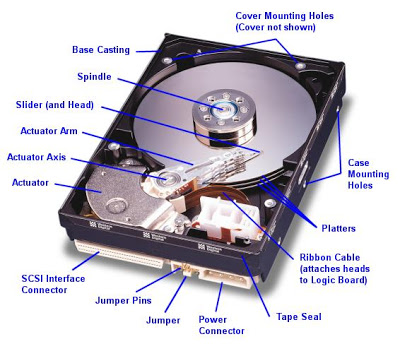
\includegraphics[width=0.4\textwidth]{images/hard-drive}
  \caption{The structure of a `traditional' spinning disk Hard Drive}
  \label{hard-drive}
\end{wrapfigure}

Hard drives consist of multiple magnetic disks (platters) laid on top of each
other that spin around and can be written to or read from by a `head'. Each
platter can store around $2\si{\tera\byte}$ at the moment, and hard drives often
have around four of them, meaning that the largest hard drives can store about
$8\si{\tera\byte}$ of data. The platters rotate at one of four speeds, $5400RPM,
7200RPM, 10000RPM$ or $15000RPM$.

Hard drives are power hungry devices compared to lots of other components in the
computer since they need power for spinning the platters, moving the heads,
reading and writing, the chips on the hard drive that control the IO etc.

Hard drives are very slow in terms of data bandwidth and latency compared to
other forms of memory storage such as RAM. The following terms are used to
quantify hard drive performance characteristics (refer to Figure~\ref{hd-config}
if you've not heard of some of the terminology before):

\begin{description}
  \item \textbf{Seek Time}:\\
    This is the time it takes for the head to reach the target track on the
    platter.
  \item \textbf{Search Time}:\\
    This is the time for the target sector to arrive under the head.
  \item \textbf{Transfer Rate}:\\
    This is the amount of data that can be read per unit time. It depends on
    a lot of factors such as where data is on the disk and access patterns of
    the data.
  \item \textbf{Disk Access Time}:\\
    The total time it takes to access data on the disk:
    \[
     \text{Disk access time} = \text{Seek time} + \text{Search time}
                                + \text{Transfer time}
    \]
\end{description}

It is sometimes important to compute the average access time of a hard drive
given the seek time, rotation speed, transfer speed and sector size. For
example, if a sector is $512\si{\byte}$, the seek time is
$8.5\si{\milli\second}$, the disk rotates at $7200RPM$ and the transfer speed is
$177\si{\mega\byte\per\second}$, then we can compute the access time to be:

\marginpar{This assumes that the hard drive will have to do $0.5$ rotations to
reach the correct sector (this is the average number of rotations when you think
about it).}

\[
  \begin{split}
    \text{Search Time (\si{\milli\second})} &= \frac{0.5\text{rotations} \times 60}{7200RPM}\\
                                            &= 4.16\si{\milli\second}\\
    \text{Transfer Time (\si{\milli\second})} &= \frac{512\si{\byte}}{177\times10^6\si{\byte\per\second}}\\
                                              &= 2.89\si{\micro\second}\\
    \text{Disk access time} &= \text{Seek time} + \text{Search time}
                                + \text{Transfer time}\\
                            &= 8.5\si{\milli\second} + 4.16\si{\milli\second} + 2.89\si{\micro\second}\\
                            &= 12.66\si{\milli\second}
  \end{split}
\]

\begin{figure}
  \centering
  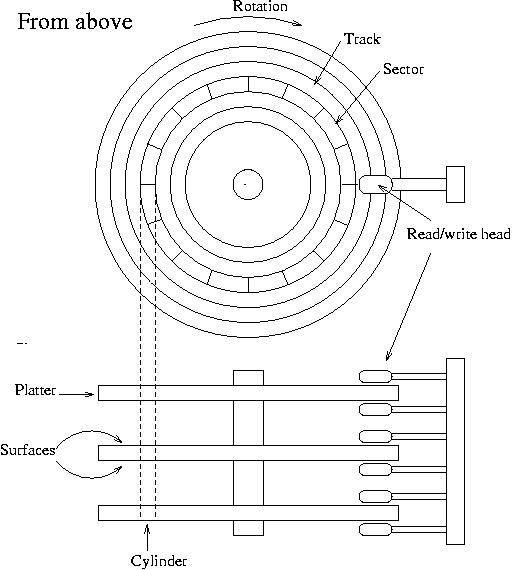
\includegraphics[width=0.5\textwidth]{images/hd-schematic}
  \caption{The internal structure of a hard drive and the layout of its disk.}
  \label{hd-config}
\end{figure}

\marginpar{See slides 9-14 on the first of the storage lecture notes for a
pictorial example.}

Sometimes, when the Operating Systems wants to read a file off the hard disk,
the file will be split over multiple sectors. In order to read the file, the
hard drive will need to move to the head to each sector to read the whole file.
If the sectors are physically distant from each other (say one was on the very
inner track of the disk, and one was on the outermost track), then the hard
drive may have to `waste' rotations in order to move the head to the correct
track. An internal processor in the hard drive will re-order the Operating
System's sector requests so that they are in the most efficient order for
retrieval.

\subsubsection{RAID}

RAID stands for a Redundant Array of Independent Disks, which is a type of
storage virtualization.

Hard disks are often too slow because of a high seek time, a high search time
and a low sustained transfer rate. We can combat the first two problems by
having multiple platters on the disk so there are more sectors per cylinder (so
the head has to move less), and increasing the speed of rotation will decrease
the search time.

A low sustained transfer rate cannot be easily increased though. One solution is
to \textit{stripe} a file over multiple disks. This is called \texttt{RAID 0}.
If a file can be split up into nine sections, we could put it on four disks like
so, and speed up our sustained transfer rate by around four times:

\begin{figure}[H]
  \centering
  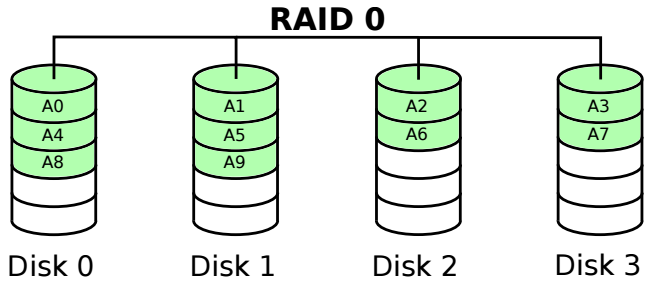
\includegraphics[width=0.6\textwidth]{images/raid0}
  \caption{RAID 0 gives higher speed, but lower reliability.}
  \label{raid0}
\end{figure}  

If a disk did break in this situation, then it'd be bad since whole swathes of
the file would disappear.

To avoid this, we could use \texttt{RAID 1}, which mirrors the data onto
another disk. This means we would have four copies of the same data, but
\textit{all} of our hard drives would have to fail before we lost any data:

\begin{figure}[H]
  \centering
  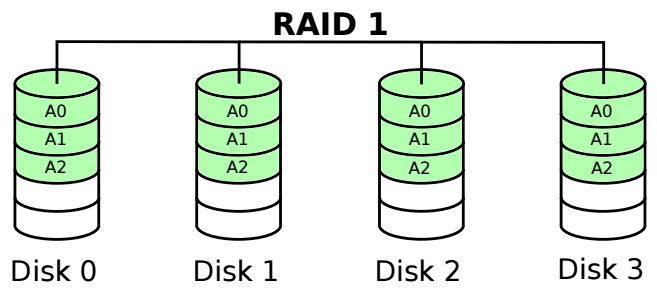
\includegraphics[width=0.6\textwidth]{images/raid1}
  \caption{RAID 1 doesn't increase speed, but it does increase reliability}
  \label{raid1}
\end{figure}

A half-way-house solution between these two, would be \texttt{RAID 10}. This is
a nested configuration, which still stripes the data, but keeps copies of the
stripes. It can tolerate disk failure as long as no mirror loses all of its
drives:

\begin{figure}[H]
  \centering
  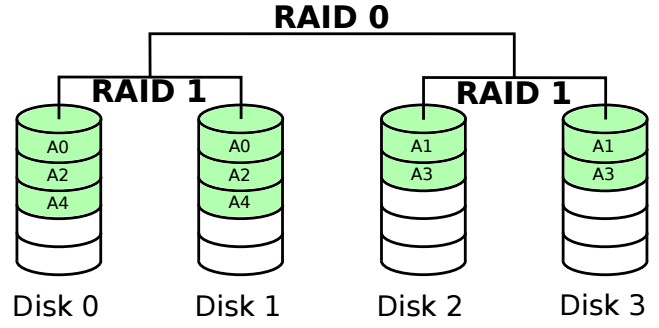
\includegraphics[width=0.6\textwidth]{images/raid10}
  \caption{RAID 10 gives higher speed, and higher reliability.}
  \label{raid10}
\end{figure}  
